\documentclass[a4paper,11pt,uplatex]{jsbook}

%\usepackage{fancyhdr}
\setlength{\footskip}{16pt}
\usepackage{amsmath}
\usepackage[dvipdfmx]{graphicx}
\usepackage[dvipdfmx]{color}
%\usepackage{pagecolor}[white]
\usepackage{amsmath,amssymb}
%\usepackage[top=3cm, bottom=3cm, left=3cm, right=3cm]{geometry}
\usepackage{braket}
\usepackage{bm}
\numberwithin{equation}{section}
\usepackage{mathrsfs}
\usepackage{siunitx}
\usepackage{physics}
\usepackage[dvipdfmx]{graphicx}
\usepackage[compat=1.1.0]{tikz-feynhand}
\usepackage{caption}
\usepackage{subcaption}
%\usepackage{cleveref}
\usepackage{float}
\usepackage{multicol}
\setlength{\columnsep}{15mm}
%\usepackage[style=phys,articletitle=false,biblabel=brackets,chaptertitle=false,pageranges=false]{biblatex}
%\usepackage[style=phys]{biblatex}
\usepackage[dvipdfmx]{hyperref}
\usepackage{url}
\usepackage{pxjahyper}
\usepackage{bookmark}
%\usepackage[backref]{hyperref}
\setcounter{tocdepth}{3}
\setlength{\parindent}{2em}
\def\vector#1{\mbox{\boldmath $#1$}}
\def\slash#1{\not\!#1}
\def\slashb#1{\not\!\!#1}
\def\delsla{\not\!\partial}
%\usepackage[dvipdfmx]{xcolor}


\hypersetup{
 setpagesize=false,
 bookmarksnumbered=true,%
 bookmarksopen=true,%
 colorlinks=true,%
 linkcolor=black,
 citecolor=red,
 urlcolor=black,
}
%backreferenceのカスタマイズ. "Back to p.3"のように表示する.
%\renewcommand*{\backref}[1]{(p.#1へ戻る)}
%\newcommand{\backtoc}{\hyperlink{toc}{[目次へ]}}
\newcommand{\backtoc}{\texorpdfstring{\protect\hyperlink{toc}{\hspace{5pt} \scriptsize [目次へ]}}{}}
\newcommand{\mychapter}[1]{\chapter[#1]{#1\backtoc}}
\newcommand{\mysection}[1]{\section[#1]{#1\backtoc}}
\newcommand{\mysubsection}[1]{\subsection[#1]{#1\backtoc}}
% 数式
%\usepackage{amsmath,amsfonts}
%\usepackage{bm}
%\usepackage{physics}
%\usepackage{siunitx}
% 画像
%\usepackage[dvipdfmx]{graphicx}
%\usepackage[dvipdfmx,colorlinks=true,linkcolor=blue]{hyperref}
%\usepackage{pxjahyper}

\begin{document}

\chapter{導入}
本論文は、ドイツ、マインツ大学にある連続電子線加速器マインツマイクロトロン(MAMI)における200 MeV領域の電子ビームエネルギー測定について論じる。
電子ビームエネルギーの絶対値を$\delta \text{E}/\text{E} \sim 10^{-4}$の精度で測定し、磁気運動量スペクトロメータの系統誤差を$\delta p/p \sim 10^{-4}$に抑えることで、
過去に我々が測定した$^4_{\Lambda} \text{H}$における$\Lambda$粒子の束縛エネルギーの精度$70$ keVから向上させ、
ハイパートライトン$^3_{\Lambda}\text{H}$における$\Lambda$束縛エネルギーを10 keVを切る精度で決定することを目指す。
ハイパートライトンにおける$\Lambda$束縛エネルギーの決定精度向上は、まだ謎の多い$\Lambda$N相互作用に対しさらなる知見を与える。

本章でははじめにハイパー核とその研究の歴史、ハイパー核生成実験について述べる。次に我々がマインツマイクロトロンにおいて独自に開発した$\Lambda$ハイパー核精密質量分光手法である
崩壊パイ中間子法とその課題となっている電子ビームエネルギー測定精度の重要性について述べた後、最後に本研究の目的を述べる。
\section{ハイパー核}

\subsection{ハイペロンとハイパー核}
素粒子の標準理論によれば、自然界の粒子は全てそれ以上分割できない最小単位の粒子(素粒子)からなり、素粒子の間に働く力は、強い力、弱い力、電磁気力、重力の4種類の力であると理解されている。
素粒子は物質を構成する粒子と力を媒介する粒子に分類でき、さらに物質を構成する粒子は強い相互作用をするクォークと強い相互作用をしないレプトンに分類できる。
クォークは表\ref{tab:quark}に示すように三世代に分類されている。
\begin{table}[t]
\centering
\begin{tabular}{c||c|c|c||c|c}
  \hline
  & 1世代 & 2世代 & 3世代 & 電荷 & スピン\\
  \hline\hline
  クォーク & u & c & t & $+2/3$e & 1/2\\
  & d & s & b & $-1/3$e & 1/2\\ \hline
  レプトン & e& $\mu$& $\tau$& $-$e& 1/2\\
  &$\nu_e$ & $\nu_\mu$& $\nu_\tau$& 0 & 1/2\\
  \hline
\end{tabular}
\caption{クォークとレプトンの一覧}\label{tab:quark}
\end{table}

クォークは単体で存在することはできず、一般に3つ集まったバリオンか2つ集まったメソンの形で存在する。我々の身の回りの物質はハドロンである陽子と中性子からなる原子核と、その周りを囲む電子からなる原子によって構成されている。
陽子、中性子は特に通常原子核を構成する意味で核子(nucleon)と呼ばれている。

構成子クォークモデルでは、陽子はuudクォーク、中性子はuddクォークからなり、それぞれ電荷+1と0を持つ。クォークにはそれぞれアイソスピンと呼ばれる量子数を導入することでスピン演算子と同じ枠組みで扱うことができることが知られている。
%荷電対称性 pp nn核力はほぼ等しい
uクォーク、dクォークはそれぞれアイソスピンの$z$成分として+1/2、$-$1/2を持ち、陽子、中性子は+1/2、$-$1/2を持つ。強い相互作用はアイソスピンのSU(2)空間回転に対してほとんど対称であることが知られている。
u、dクォークのSU(2)対称性にsクォークを加えて拡張したSU(3)対称性は、u、dクォークに比べてsクォークが比較的重く、疑似的な対称性とみなされている。
これらu、d、sクォークからなるバリオンはフレーバーSU(3)の枠組みにおいて、スピン1/2のバリオン8重項、スピン3/2のバリオン10重項に分類される(図\ref{fig:baryon})。
一方でc,b,t クォークはu,d,sクォークと比較すると極端に重いため、SU(N)の対称性が破れる。
\begin{figure}[h]
  \centering
  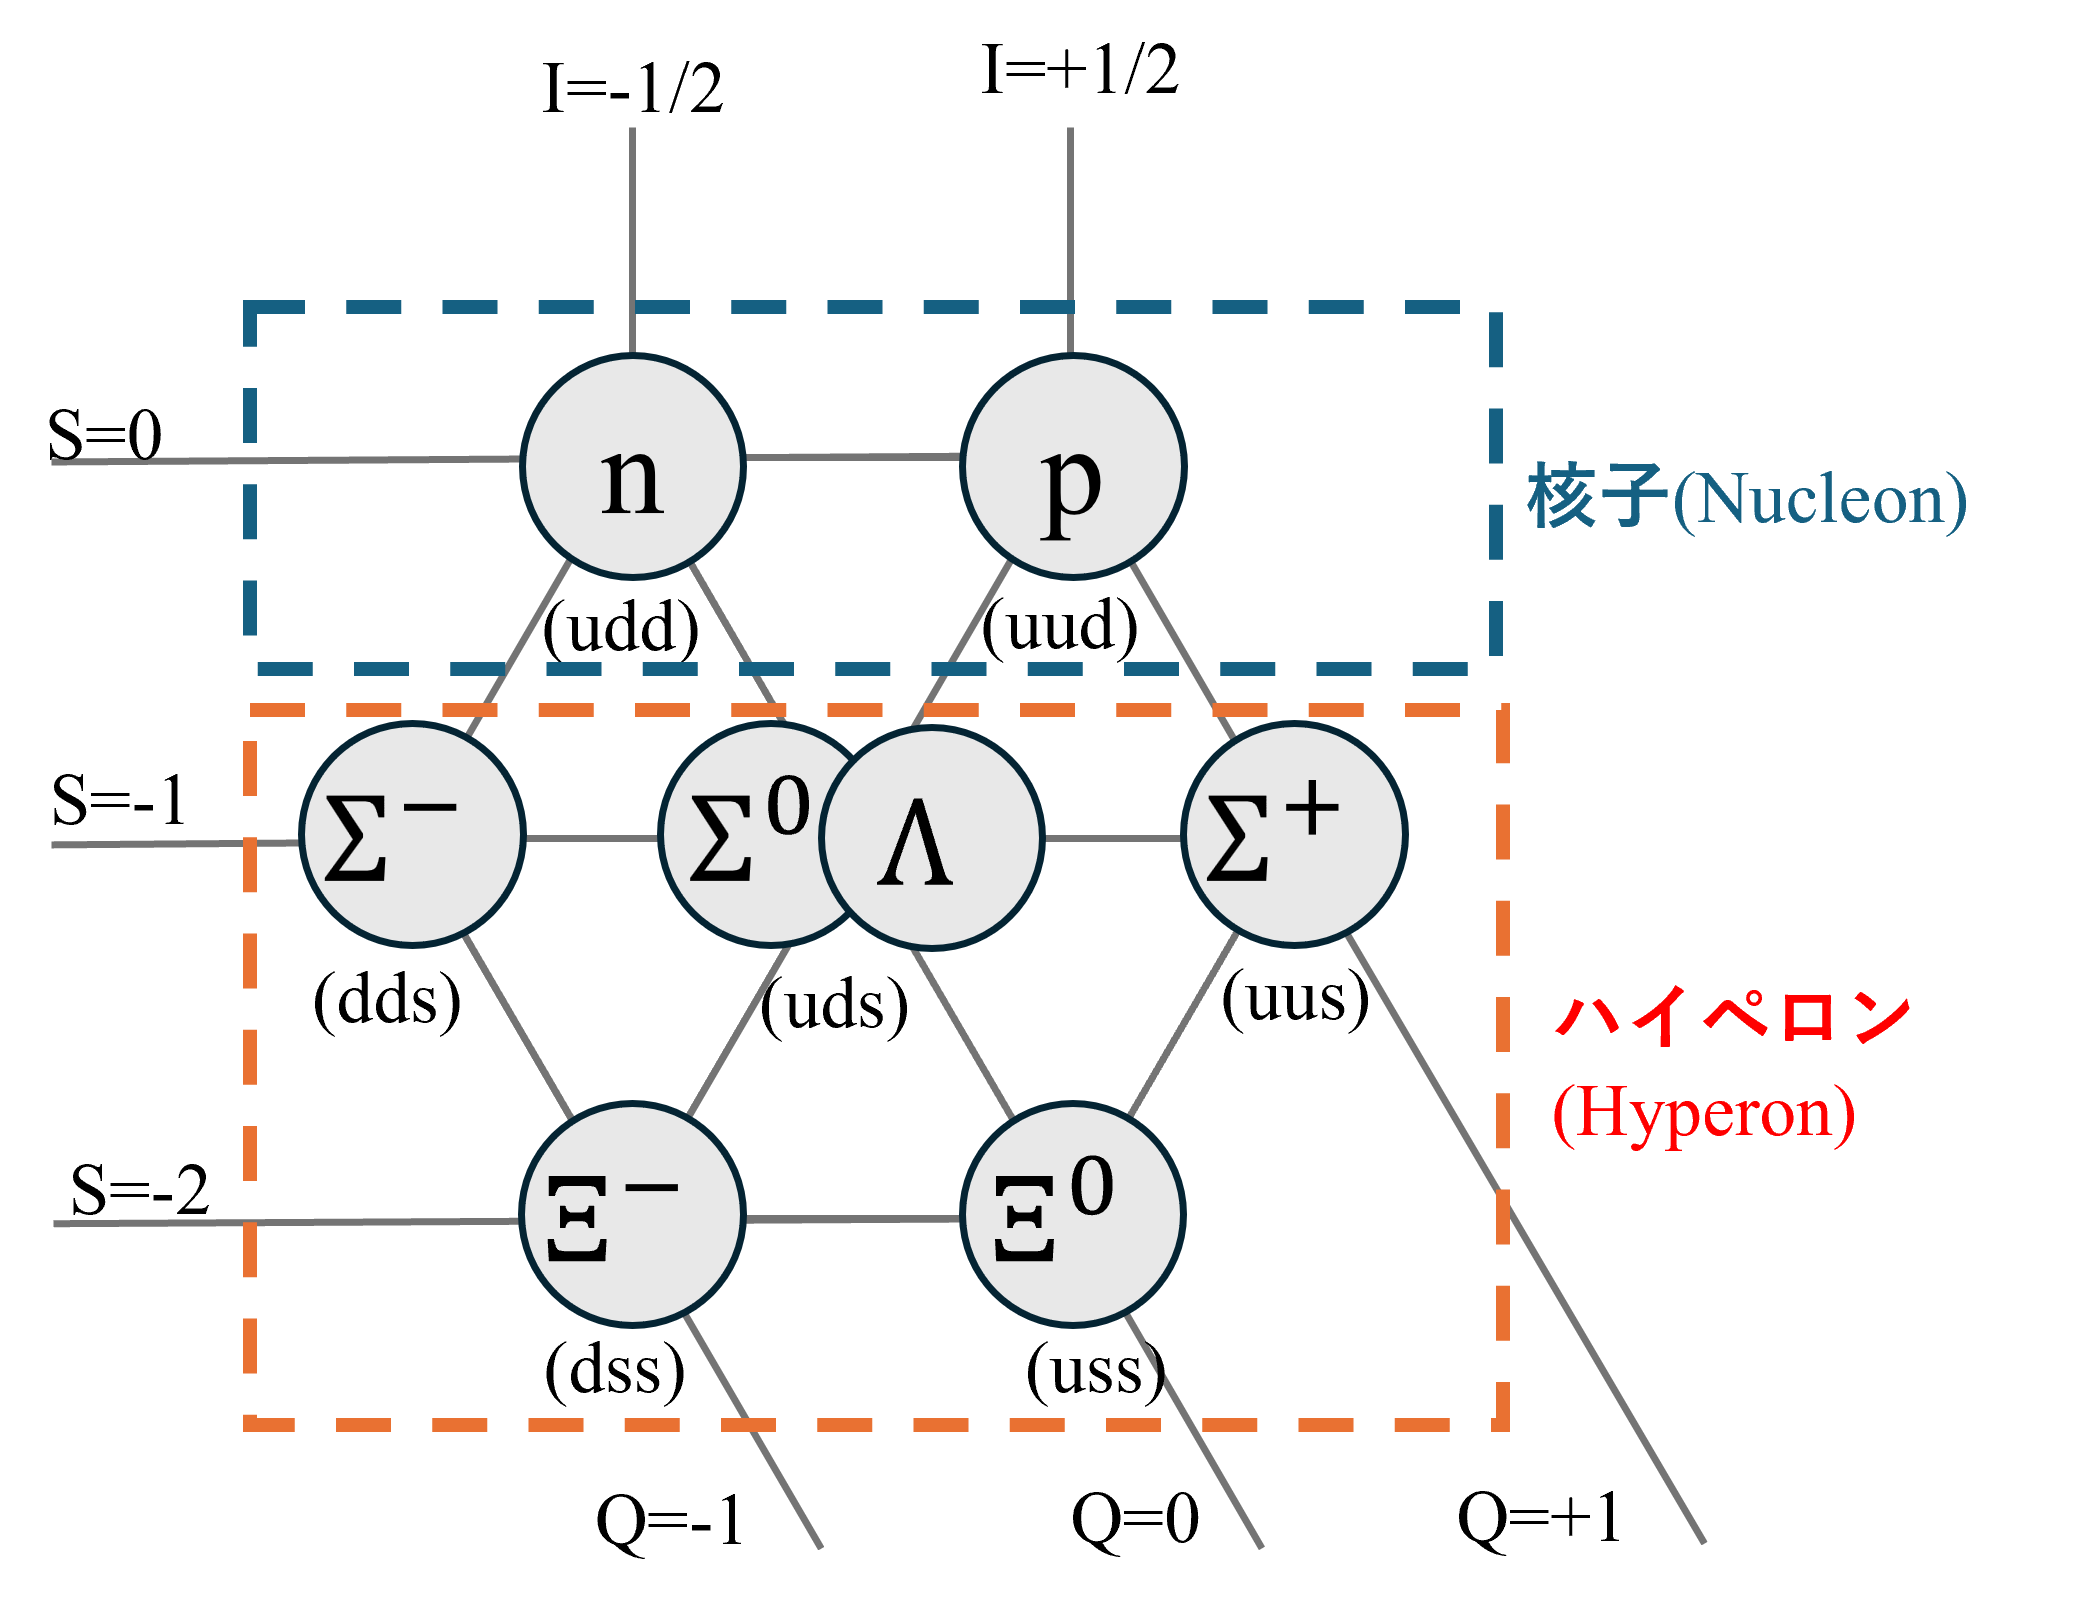
\includegraphics[width=10cm]{image/1_baryon.png}
  \caption[バリオン8重項]{バリオン8重項。アイソスピンI、電荷Qに加え、ストレンジネスSの計3つの量子数を示した}
  \label{fig:baryon}
\end{figure}

特にsクォークを含むバリオンをハイペロンと呼ぶ。その中でもu、d、sクォークからなるΛ粒子は最も軽い基本的なハイペロンである。
\begin{table}[h]
\centering
\begin{tabular}{c||cccc}
  \hline
  ハイペロン&質量(MeV/$c^2$)&寿命 (s)&主な崩壊モード&分岐比(\%)\\
  \hline \hline 
  \multirow{2}{*}{$\Lambda$} & \multirow{2}{*}{1115.683(6)} & \multirow{2}{*}{$2.632(10) \times 10^{-10}$} & $p + \pi^-$ &63.9(5)\\
                             &                              &                                              & $n + \pi^0$ & 35.8(5)\\ \hline
  $\Sigma^0$                 & 1192.642(4)                  & $7.4(7) \times 10^{-20}$                     & $\Lambda + \gamma$ & 100\\ \hline
  \multirow{2}{*}{$\Sigma^+$}& \multirow{2}{*}{1189.37(7)}  & \multirow{2}{*}{$0.799(5) \times 10^{-10}$}  & $p + \pi^0$ & 51.57(30)\\
                             &                              &                                              & $n + \pi^+$ & 48.31(30)\\ \hline
  $\Sigma^-$                 & 1197.45(7)                   & $0.486(5) \times 10^{-10}$                   & $n + \pi^-$ & 99.848(5)\\ \hline
\end{tabular}
\caption[代表的なハイペロンの性質]{ハイペロンの性質。数値の末尾に付けた括弧は統計誤差を表す\cite{Beringer}。}
\end{table}

原子核中に核子だけでなくハイペロンを含む原子核をハイパー核と呼ぶ。ハイパー核には通常核子には見られない性質が現れることが知られており、それ自体が重要な研究対象である。
ここではハイパー核の性質の一つとして、崩壊モードについてこの章で詳しく述べる。
%λΣの表の説明を本文にも入れる
自由空間では$\Lambda$粒子の寿命は$10^{-10}$秒程度で、$\pi$中間子を放出して崩壊する。これは中間子弱崩壊と呼ばれる。

一方$\Lambda$粒子が原子核に束縛されている$\Lambda$ハイパー核の場合には、中間子弱崩壊で$\pi$中間子とともに放出された核子が、原子核の他の核子の影響を受けてフェルミの排他律を受けることにより、中間子弱崩壊が抑制される。
その結果、中間子を放出しないような崩壊、いわゆる非中間子弱崩壊が主な崩壊モードとなる。

軽いハイパー核の場合には核子によって占められているフェルミ準位が低いため、重いハイパー核と比較すると中間子弱崩壊が起こりやすいと言える。

他にもハイペロンとして$\Sigma$粒子や$\Xi$粒子がある。$\Sigma$粒子は核子との相互作用が斥力的であることが知られており、束縛系を作ることが困難であるため
散乱実験が有力な研究方法となる。また$\Xi$粒子は過去に$\Xi$ハイパー核を生成する実験が行われた\cite{fukuda,khaustov}が、統計と分解能が不十分であった。
現在はJ-PARCで$\Xi$ハイパー核を生成する実験が行われている。

\subsection{ハイパー核研究の意義}
この節では特に$\Lambda$ハイパー核に焦点をあててハイパー核研究の意義について述べる。
ハイパー核研究において、通常核子間の核力(NN相互作用)に加えてハイペロンと核子の相互作用(YN相互作用)を調べることができる。
ハイパー核の研究では、このYN相互作用の知見を得ることが一つの重要なモチベーションとなっている。

YN相互作用に関する重要な研究テーマにはハイペロンパズル、荷電対称性の破れ、ハイパートライトンパズル等がある。
\subsubsection{ハイペロンパズル}
中性子星内部では中性子のフェルミエネルギーが$\Lambda$粒子の生成エネルギーを上回るため、$\Lambda$粒子が生成されるという理論予想が提唱されている\cite{Ambartsumyan}。
従って、中性子星内部の状態方程式には$\Lambda$N相互作用の項が自然に含まれると考えられる。
現在の$\Lambda$N相互作用の理解に基づく状態方程式によると、中性子星の質量は太陽質量の2倍よりも大きくなることはないとされている\cite{schulze}。
しかし近年、宇宙観測によって太陽質量の2倍以上の質量をもつ中性子星(PSR J1614-2330\cite{demorest2010}, PSR J0348+0432\cite{antoniadis2013},PSR J740+6620\cite{cromartie2019})が観測された。この宇宙観測と理論予測の矛盾が「ハイペロンパズル」と呼ばれ、ハイパー核研究の重要な問題になっている。
ハイペロンパズルの解決には$\Lambda$N相互作用のより正確な知見が不可欠であり、三体バリオン斥力を用いたモデル計算\cite{yamamoto2014}などがハイペロンパズルの解決の糸口を提供しているが、同時に実験的な検証が求められている状況である。

\subsubsection{荷電対称性の破れ}
NN相互作用においては、クーロン力の効果を除いた核力は荷電対称性を持つ。すなわち、陽子$-$陽子間に働く力と中性子$-$中性子に働く力は核力においてほとんど区別されない。特に質量数A=3程度の軽い原子核において、実験と理論の両側面から荷電対称性の破れは数 keVの精度で理解されている\cite{Audi,NagaoD,friar1970, coon}。

一方で$\Lambda$粒子と核子間の相互作用には荷電対称性の破れが存在することが実験的に検証された。$^4_\Lambda \text{H}$と$^4_\Lambda \text{He}$
のA=4体系のハイパー核において、2012年に我々の研究グループが行ったハイパー核分光実験によって$^4_\Lambda \text{H}$の基底状態における$\Lambda$粒子束縛エネルギーを$B_\Lambda = 2.12 \pm 0.01 (\text{stat.} \pm 0.09 (\text{sys.}))$~MeVと決定した\cite{esserObservation4Hyperhydrogen2015,NagaoD}。
またJ-PARCで行われたハイパー核$\gamma$線分光実験では、$^4_\Lambda \text{He}$が$1^+$状態から$0^+$状態に遷移する時に放出される$\gamma$線を測定し、
$E_\gamma = 1.406 \pm 0.002(\text{stat.}) \pm 0.002 (\text{sys.})$~MeVと決定した\cite{yamamoto2015}。この結果と過去の原子核乾板実験の結果から、
基底状態の束縛エネルギーの差が$\Delta B_\Lambda = B_\Lambda(^4_\Lambda\text{H}) - B_\Lambda(^4_\Lambda\text{He}) = -270 \pm 90$~keVと得られた。
この値は$^3\text{H}$,$^3\text{He}$の強い相互作用による束縛エネルギーの差やクーロン力でも説明できない$\Lambda$N相互作用における荷電対称性の破れとして理解されている。

A=4程度の少数多体系においても、$\Lambda$N相互作用の荷電対称性の破れは依然として理解が不十分であり、軽い$\Lambda$ハイパー核における束縛エネルギーの
精密測定の重要性は非常に高い。J-PARCではA=7体系における荷電対称性の破れの測定が進行中である。
\subsubsection{ハイパートライトンパズル}
ハイパートライトンは陽子、中性子、$\Lambda$からなるA=3体系のもっとも基本的な$\Lambda$ハイパー核である。
前節で軽いハイパー核の研究の重要性について述べたが、ハイパートライトンパズルの重要性については\ref{sec:hypertriton puzzle}章で詳しく述べる。
\subsubsection{原子核深部のプローブ}
ハイパー核研究の目的はYN相互作用の測定だけにとどまらない。
ハイペロンは核子とは量子数の異なる粒子であるためパウリの排他律を受けず、エネルギー準位の低い(深い)軌道にも束縛される。
このため、ハイパー核内での$\Lambda$粒子のエネルギー準位を調べることによって、原子核深部の情報を得ることができる。
また、原子核深部におけるバリオンの振る舞いの統一的な理解に役立つほか、$\Lambda$粒子を入れることで原子核構造を変化させることができる点もハイパー核研究の魅力である。

\subsection{ハイパー核質量分光}
YN相互作用を実験的に調べる手法の一つが質量分光である。これはハイパー核を生成し、その質量を測定する実験手法を指す。分光実験には様々な手法があるが、特にハイパー核の生成方法と、
生成したハイパー核の質量を決定する方法でそれぞれ分類することができる。

ハイパー核の生成反応は主に$(K^-, \pi^-)$反応、$(\pi^+, K^+)$反応、$(e,e'K^+)$反応がある(図\ref{fig:production})。
\begin{figure}[h]
  \centering
  \begin{subfigure}[b]{0.47\linewidth}
    \centering
    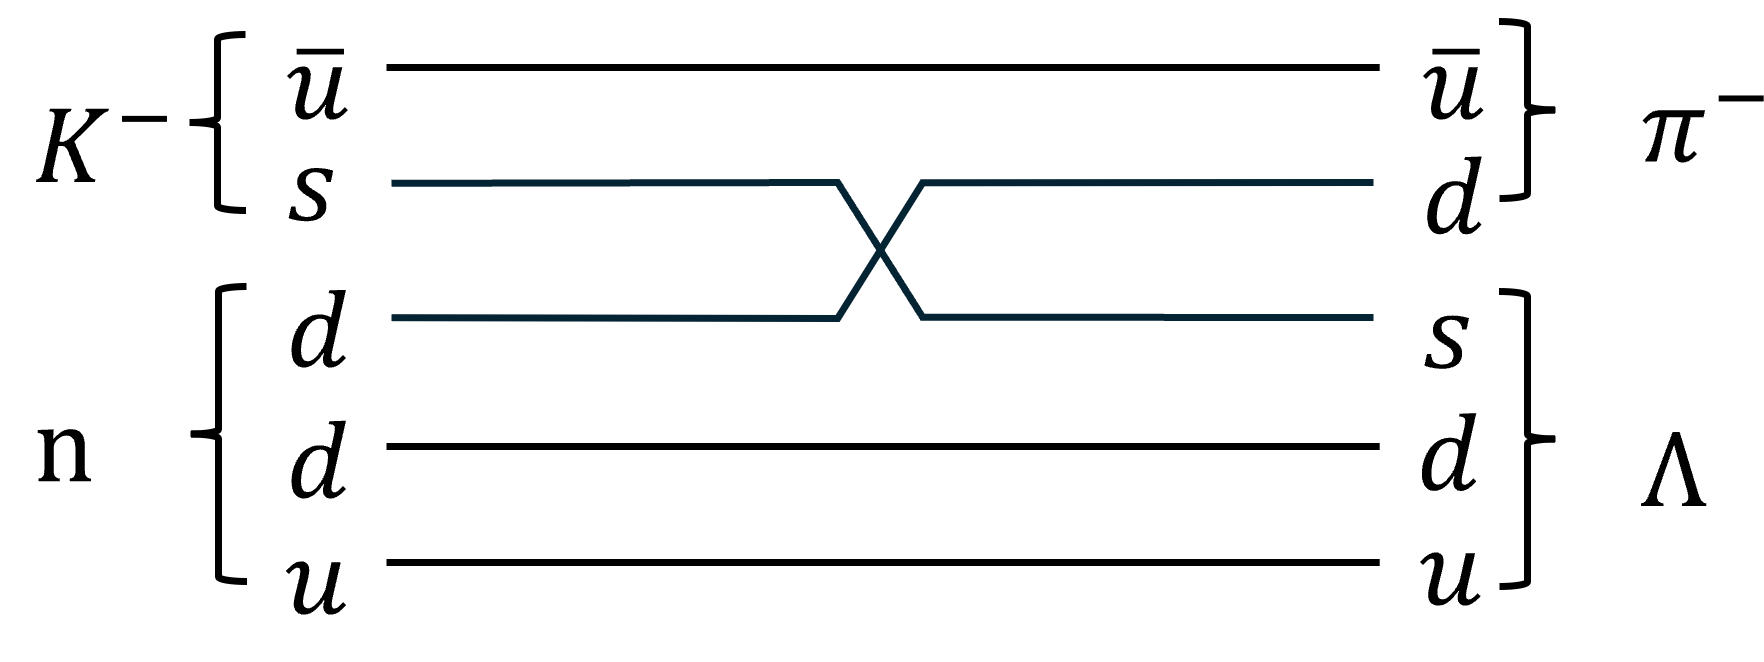
\includegraphics[width=\linewidth]{image/1-Kpi.png}
    \subcaption{($K^-, \pi^-$)反応}
  \end{subfigure}
  \hfill
  \begin{subfigure}[b]{0.47\linewidth}
    \centering
    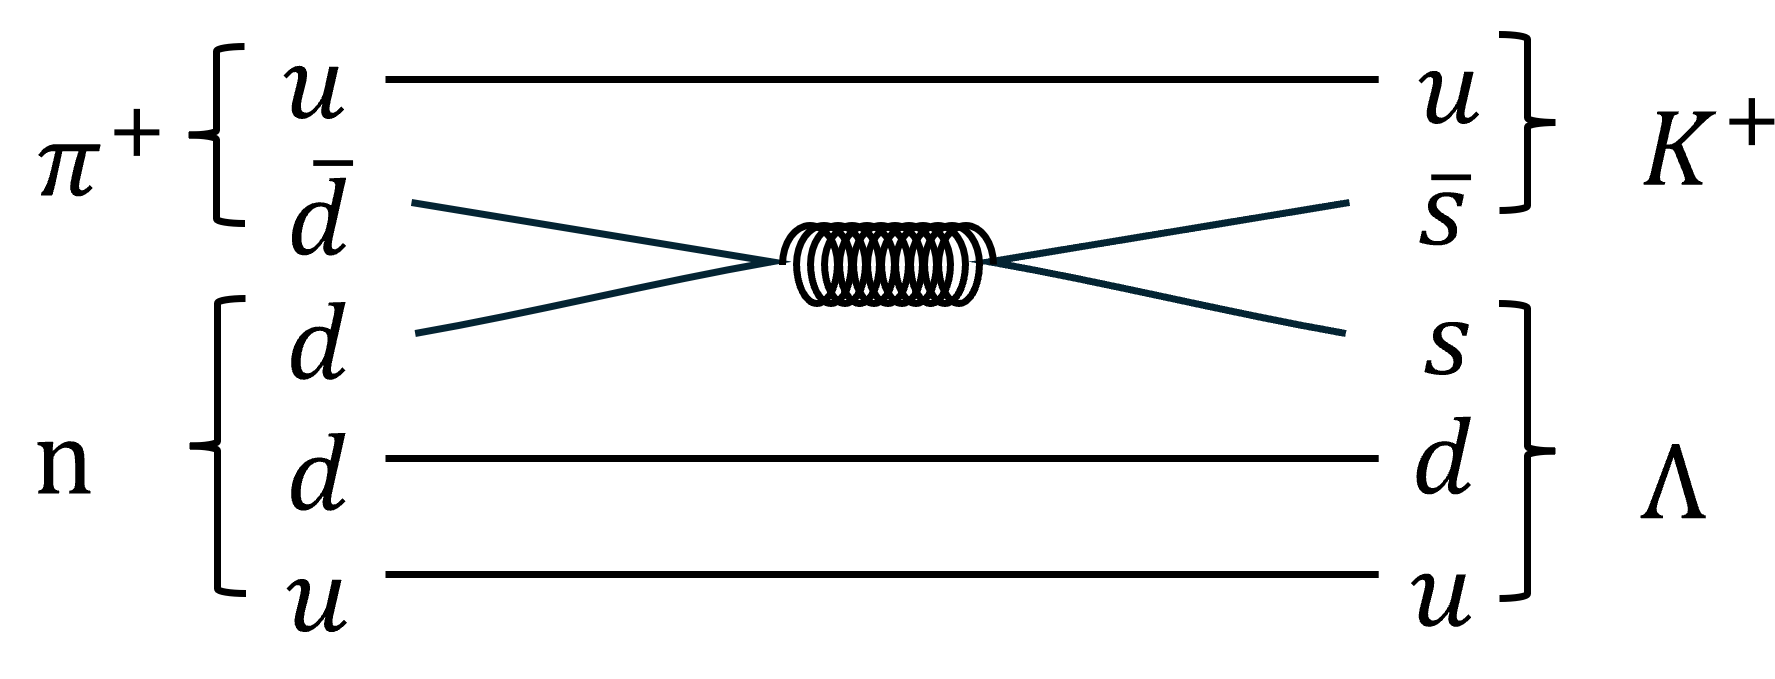
\includegraphics[width=\linewidth]{image/1-piK.png}
    \subcaption{($\pi^+, K^+$)反応}
  \end{subfigure}
  \begin{subfigure}[b]{0.5\linewidth}
    \centering
    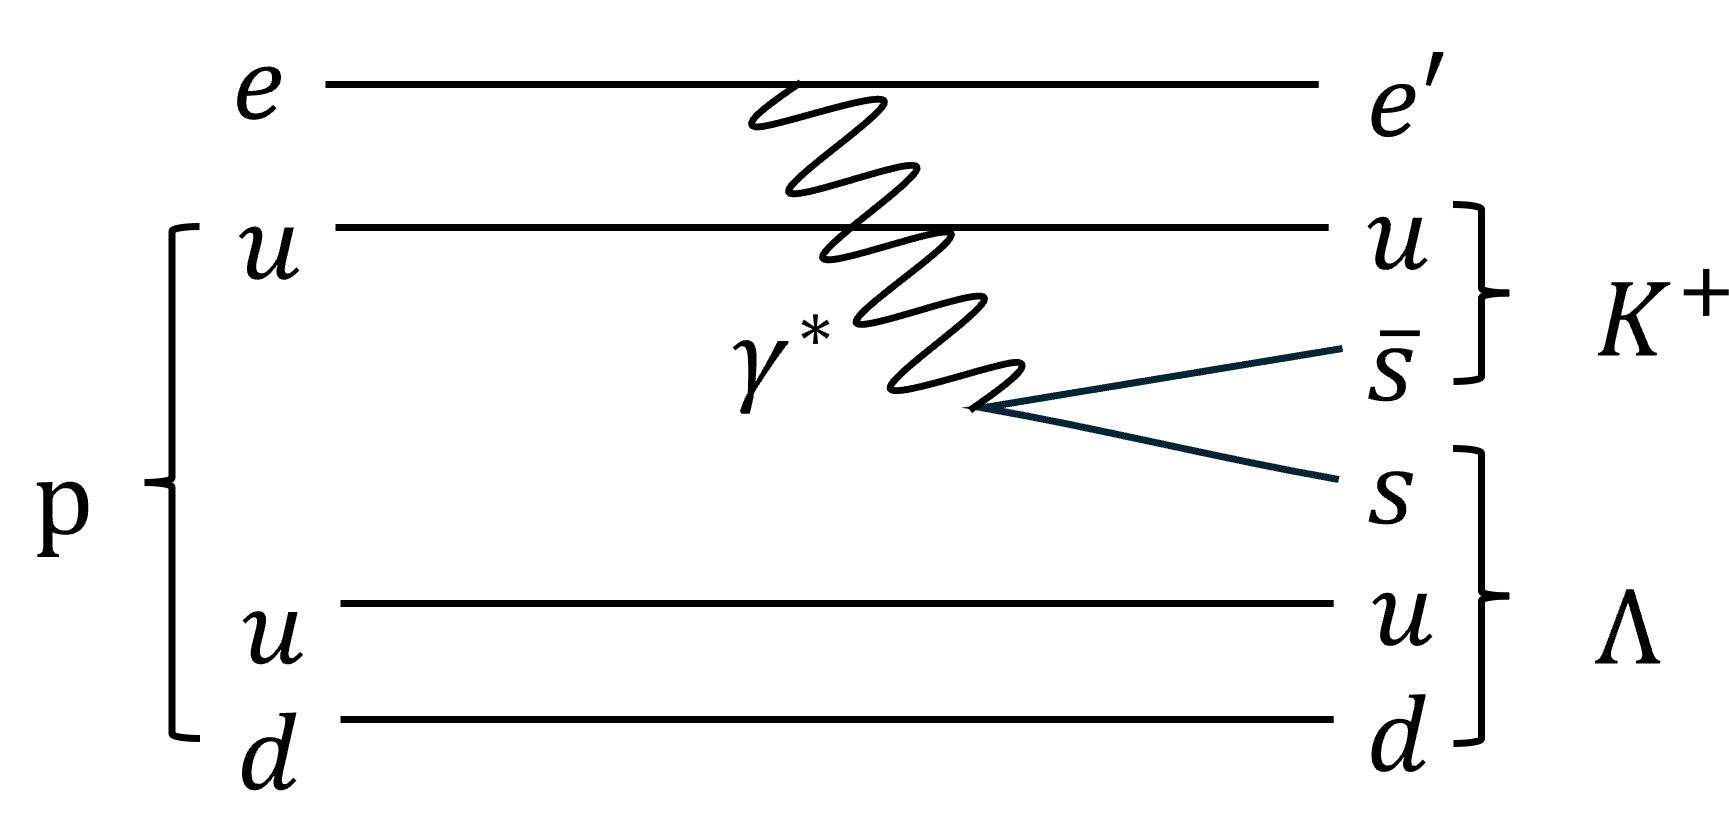
\includegraphics[width=\linewidth]{image/1-eeK.png}
    \subcaption{($e,e'K^+$)反応。$\gamma^*$は仮想光子を表す}
  \end{subfigure}
  \caption[主なハイパー核生成反応のファインマンダイアグラム]{主なハイパー核生成反応のファインマンダイアグラム}
  \label{fig:production}
\end{figure}

\subsubsection{($K^-, \pi^-$)}
クォーク交換反応である。sクォークを生成する必要がないため、他の生成反応と比較しても最もΛ粒子の生成断面積が大きい。
他の反応とは異なり発熱反応であるので静止した$K^-$からでも$\Lambda$粒子を生成することができるという点が特徴的である。
\subsubsection{($\pi^+, K^+$)}
核内で$\text{d}$,$\bar{\text{d}}$クォークが対消滅し、$\text{s}$,$\bar{\text{s}}$クォークが生成される。この反応は($K^-$,$\pi^-$)と比較するとΛ粒子の生成断面積が小さいが、
一般に$K$ビームよりも$\pi$ビームが強度の高いビームを得られるため、問題とならない。
運動量移行が大きいため、$\Lambda$が様々な軌道角運動量に入った状態を生成することができる。
\subsubsection{$(e,e'K^+)$}
電子ビームを用いて、仮想光子を媒介して$\text{s}$,$\bar{\text{s}}$クォークを生成する反応である。電磁相互作用による反応であるため3つの反応の中で最も生成断面積が小さいが、
電子ビームは高い強度が得られるため、十分な統計量を得ることができる。更に$\pi、K$といった中間子ビームは二次ビームであるのに対して、
加速器で直接加速した高品質な一次電子ビームを用いることができるため、高い分解能を得ることができる。
\vskip\baselineskip
生成したハイパー核の質量は、入射ビーム運動量及び崩壊によって生成する粒子の運動量、エネルギーを測定することで、
欠損質量法\footnote{欠損質量法は生成したハイパー核以外の入射、散乱粒子全ての運動量を測定することで、エネルギー・運動量保存則から生成した粒子のエネルギー・運動量を決定する。エネルギー・運動量が求まれば$m = \sqrt{E^2 -p^2}$によって質量を求めることができる。}や
不変質量法\footnote{不変質量法はハイパー核が崩壊して生成した全ての粒子の運動量・エネルギーを測定することによって親核のハイパー核質量を$m = \sqrt{(\sum E_i)^2 - (\sum p_i/c)^2}$として求める方法である。}などによって求めることができる。
また本研究では崩壊パイ中間子法と呼ばれる手法によってハイパー核の質量を決定している。詳細については\ref{DPS}章で述べる。
こうした質量分光では、カウンターと呼ばれる粒子検出器と高速電気信号処理装置を用いて大量のデータを取得するカウンター実験という手法が一般的である。
\vskip\baselineskip
同じカウンター実験であるが、全く異なるハイパー核生成の手法が近年注目されている。
\subsubsection{重イオン衝突実験}
原子核同士を高エネルギーまで加速させて衝突させると様々な反応が同時に起こる。これを利用してハイパー核を生成し、生成した粒子の運動量を測定することで
不変質量を計算しハイパー核の質量を決定する。
前節までの反応分光とは異なり生成可能なハイパー核の各種が標的によらず、様々なハイパー核を同時に生成することが可能である。
\vskip\baselineskip
ここまで紹介したカウンター実験と対照的な手法として原子核乾板による質量分光法がある。
\subsubsection{原子核乾板実験}
原子核乾板はアクリル板などにAgBrなどの乳剤を添付したものである。
原子核乾板中を荷電粒子が通過すると、乾板中の原子核が電離され、発生した電離電子によって乾板中の銀イオンが結合し粒子の軌跡が残る。
この軌跡を読み取ることで、粒子の識別、運動量測定を同時に行うのが原子核乾板による粒子検出法、質量分光法である。
過去には$\Lambda$粒子を2個含んだダブルハイパー核の観測に世界で初めて観測することに成功するなど\cite{takahashi2001}、まれな事象を検出するのに有効な手法である。

\subsection{ハイパートライトンパズル}\label{sec:hypertriton puzzle}
このように様々な手法によってハイパー核研究が進められる中で、近年注目を集めているテーマの一つがハイパートライトンパズルである。

ハイパー核の中でも最も基本的な束縛系が$^3_{\Lambda}\text{H}$、ハイパートライトンである。これは陽子、中性子、Λ粒子それぞれ一つずつからなるハイパー核である。
1960年代に原子核乾板や泡箱実験によってハイパートライトンにおける$\Lambda$粒子の束縛エネルギーは$B_{\Lambda} = 130 \pm 50(\text{stat.}) \pm 40(\text{syst.})$ keVとされており\cite{Juric}、この結果が約50 年間信じられてきた。
100 keV程度の弱い束縛から計算すると、Λ粒子の波動関数は鉛原子核の半径程度の広がりを持つことが示唆される。
これは陽子、中性子からなるコア核によって束縛された状態よりも、自由空間の$\Lambda$粒子に近い状態であると考えられる。%もう少し説明を加える、波動関数の半径が鉛くらい、の論文、だからほぼ自由空間のΛ粒子と同じ状態
従ってその寿命は自由空間のΛ粒子と同程度であると見積もられる。

これに対して2010年代に重イオン衝突実験が、ハイパートライトンの寿命が予測よりも有意に短いことを示唆する実験結果を次々と報告した\cite{HI-1,HI-2,HI-3,HI-4}。これらの値は$\tau \sim$200 psであり、
$B_{\Lambda} = 130$ keVの結果と整合性のある物理的な解釈はいまだない。この問題をハイパートライトンパズルと呼ぶ。

2020 年代にはSTAR,ALICEの2つの重イオン衝突実験が束縛エネルギーや寿命の測定を行っている。STAR実験\cite{STAR}は
\begin{align*}
  B_{\Lambda} = 406 \pm 120(stat.) \pm 110 (syst.) ~\text{keV}
\end{align*}
という結果を報告しているのに対し、ALICE実験\cite{ALICE}では
\begin{align*}
  \tau        &= 253 \pm 11(stat.) \pm 6(syst.) ~\text{ps},\\
  B_{\Lambda} &= 102 \pm 63(stat.) \pm 67(syst.) ~\text{keV}
\end{align*}
という結果を報告している。これらの結果を図\ref{fig:hypertriton}に示す。

ALICE実験の結果は100~keVの弱い束縛に対して寿命が253~psと従来の描像とは矛盾のない結果が得られているものの、
同じ重イオン衝突実験による2つの実験結果で異なる結果が得られていることや、$B_{\Lambda}$の統計誤差、系統誤差が100~keV程度と大きいことから、
ハイパートライトンパズルの解決には引き続き実験的な検証が求められている。特に重イオン衝突実験以外の手法による測定が重要であると考えられる。

\begin{figure}[H]
  \centering
  \begin{subfigure}{0.8\linewidth}
    \centering
    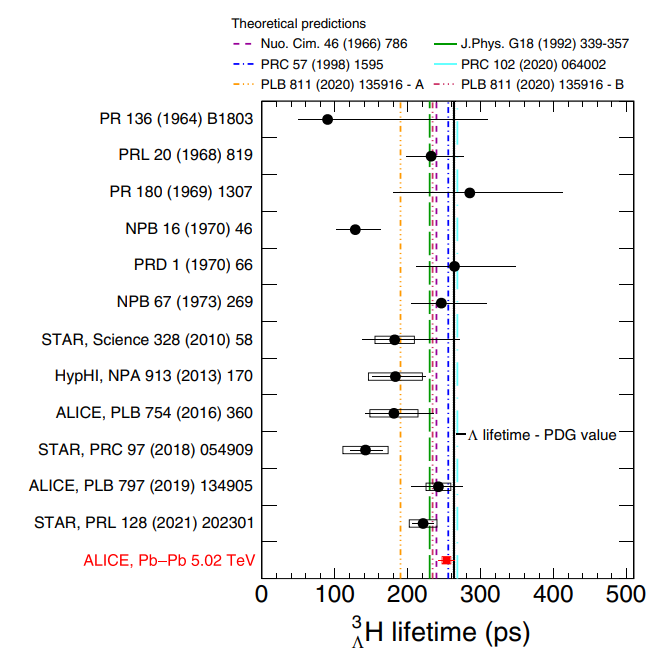
\includegraphics[width=10cm]{image/1-lifetime.png}
  \end{subfigure}
  \begin{subfigure}{0.8\linewidth}
    \centering
    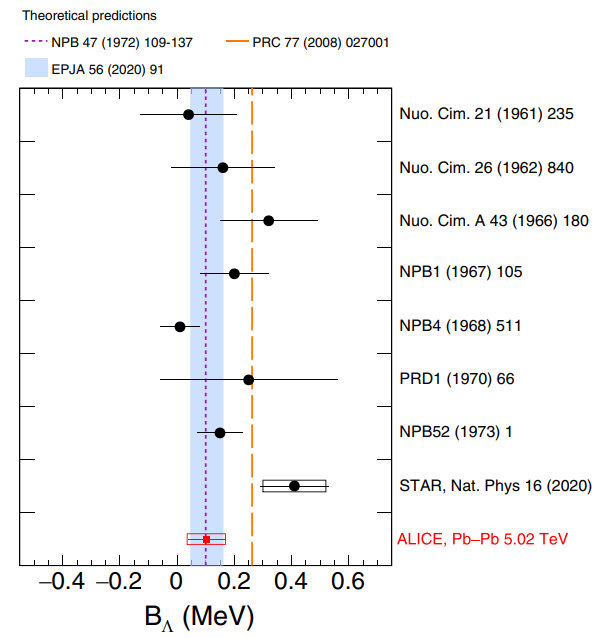
\includegraphics[width=10cm]{image/1-binding.png}
  \end{subfigure}
  \caption[過去のハイパートライトンの寿命測定及び束縛エネルギー測定実験]{過去実験によるハイパートライトンの寿命(上)、束縛エネルギー(下)の測定結果の比較。図は\cite{ALICE}より引用。}\label{fig:hypertriton}
\end{figure}

\section{崩壊パイ中間子法}\label{DPS}
崩壊パイ中間子法は2010年代にドイツのマインツ大学マイクロトロン(MAMI)で我々の研究グループによって開発されたハイパー核の質量分光法である\cite{esserObservation4Hyperhydrogen2015}。
10 keVを切る高いエネルギー分解能が実証されている\cite{Schulz2015} ため、ハイパートライトンパズルの解明に有効な手法であると期待されている。
この章では崩壊パイ中間子法の原理を述べる(\ref{sec:dps principle}節)。そして高い分解能が実現できる理由と、解決すべき課題である大きな系統誤差について述べる(\ref{sec:systematic_error})。
\subsection{原理}\label{sec:dps principle}
電子ビームで電磁生成したハイパー核が核破砕し、目的のハイパー核が標的中で静止し2体崩壊する反応を検出する。
この時ハイパー核の質量$m(^A_{\Lambda}Z)$は2体崩壊に注意すると
\begin{eqnarray}
  m(^A_{\Lambda}Z) = \sqrt{m(^A(Z+1))^2 + (p_\pi/c)^2} + \sqrt{m_\pi^2 + (p_\pi/c)^2} \label{mass formula}
\end{eqnarray}
と$\pi$中間子の運動量$p_\pi$のみで求めることができる(図\ref{fig:DPS})。
\begin{figure}[H]
  \centering
  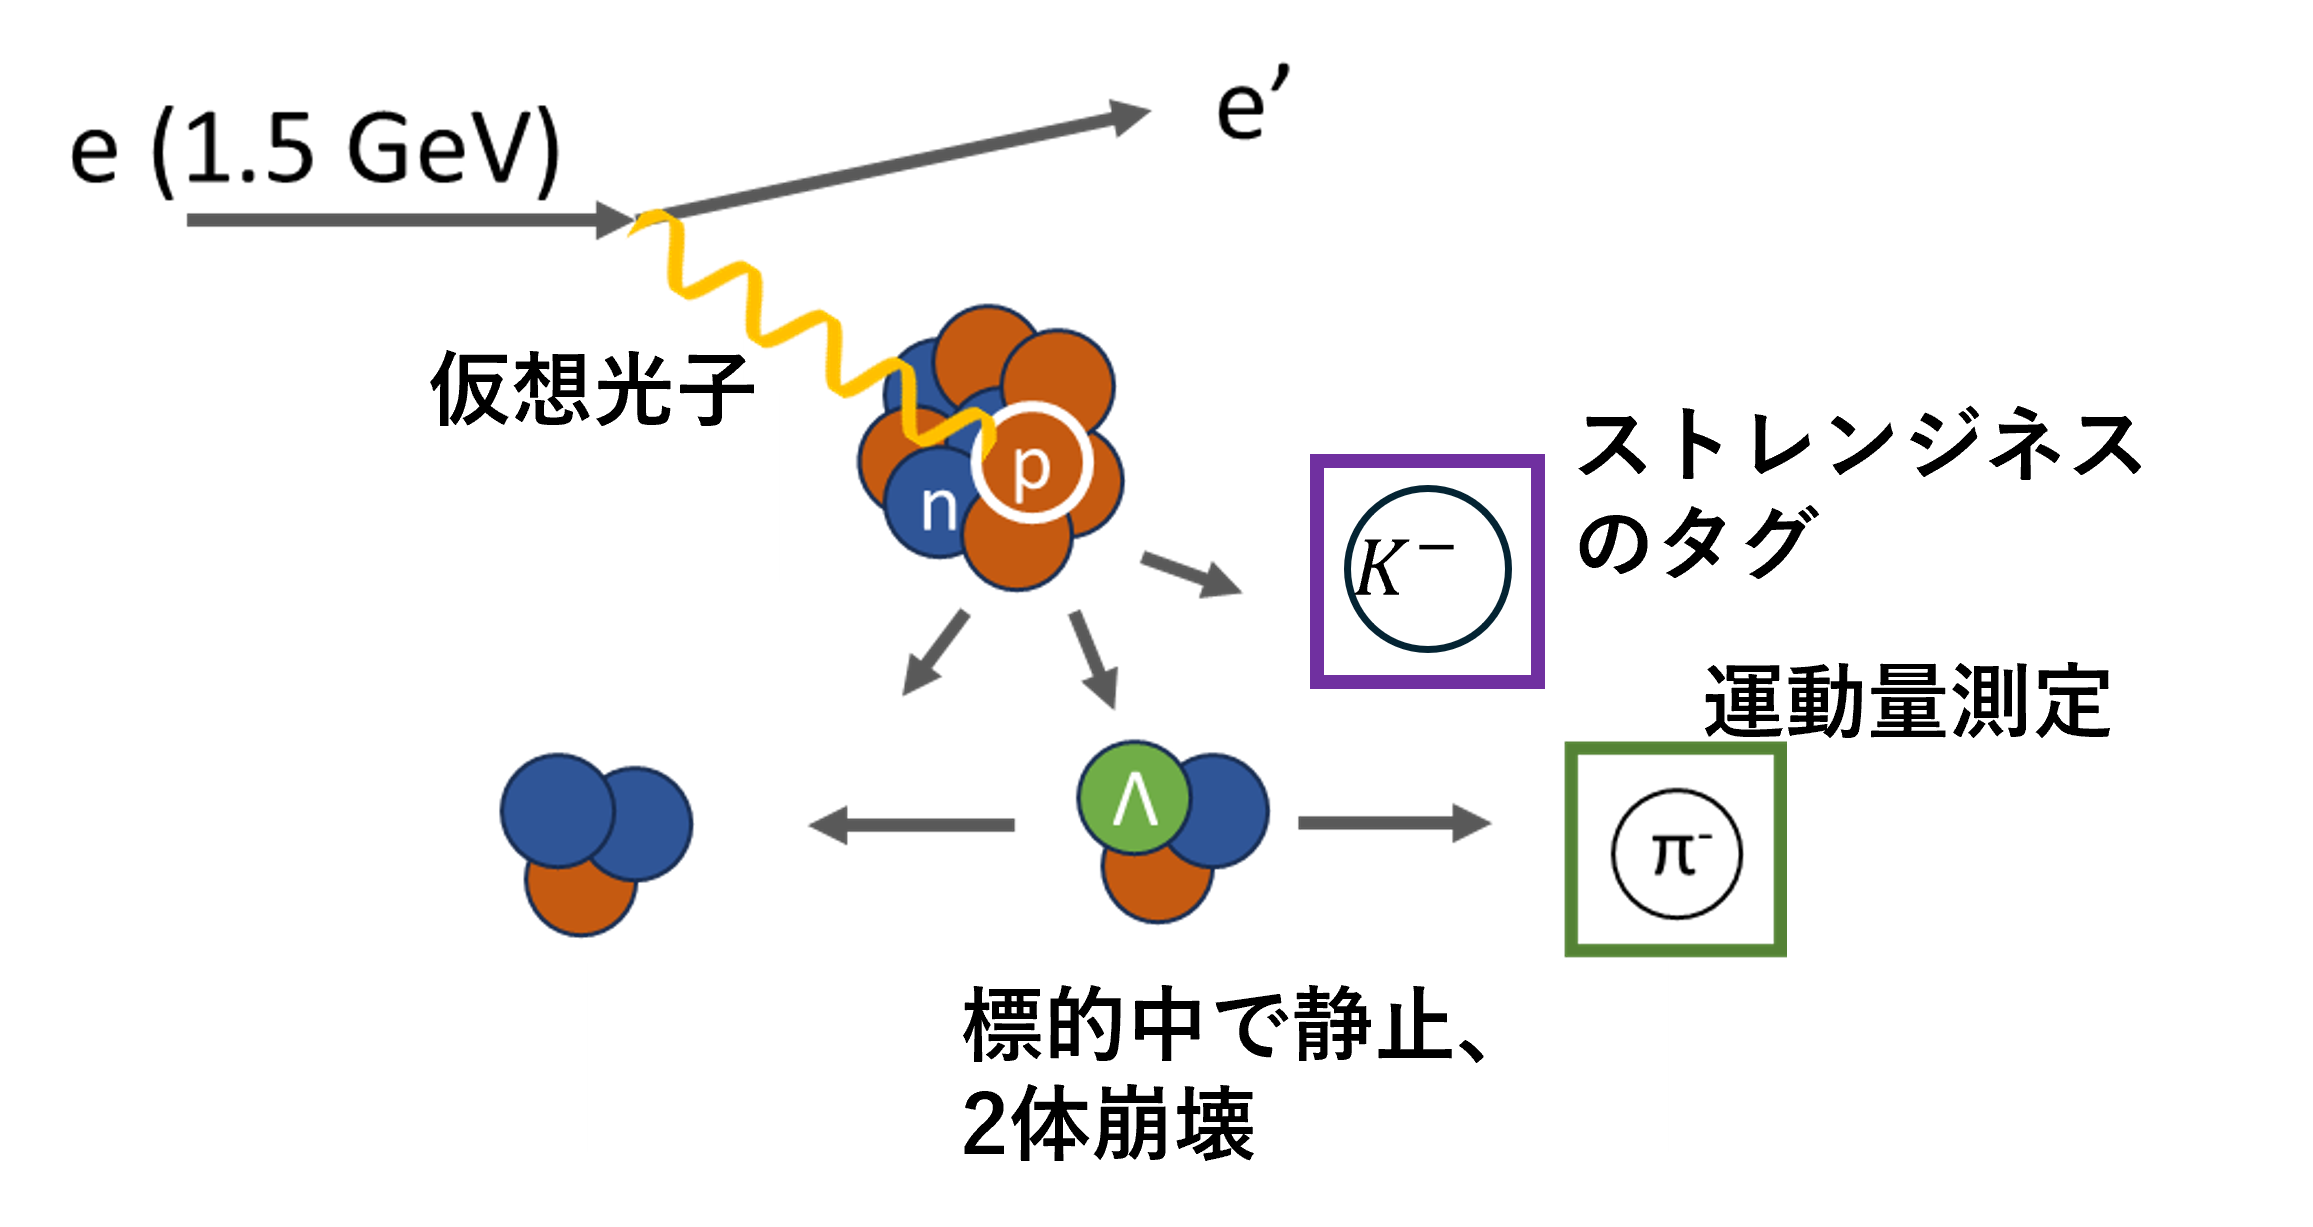
\includegraphics[width=10cm]{image/1-DPS.png}
  \caption[崩壊パイ中間子法の原理]{崩壊パイ中間子法の原理。電子ビームで生成されたハイパー核が標的中で静止したのち2体崩壊し、$\pi$中間子が放出される。
  この時$\pi$中間子の運動量を測定することでハイパー核の質量を決定する。またハイパー核が生成する際に同時に放出される$K^+$を検出することで
  $\Lambda$ハイパー核が生成されたイベントを選択することができる。}\label{fig:DPS}
\end{figure}

Λハイパー核の質量$m(^A_\Lambda Z)$からこのハイパー核における$\Lambda$粒子の束縛エネルギー$B_\Lambda$は、$\Lambda$粒子を除いたコア核の質量$m_{core}$と$\Lambda$粒子の質量$m_\Lambda$を用いて
\begin{eqnarray}
  B_\Lambda = m_{core} + m_\Lambda - m(^A_\Lambda Z) \label{binding energy formula}
\end{eqnarray}
と求めることができる。

ハイパートライトンがパイ中間子を放出する崩壊モードは
\begin{eqnarray}
  ^3_{\Lambda}\text{H} \rightarrow ^3\text{He} + \pi^-
\end{eqnarray}
であるから、式(\ref{mass formula})、式(\ref{binding energy formula})より、$m(^3_\Lambda\text{H})$と$B_\Lambda$は
\begin{eqnarray}
  m(^3_\Lambda \text{H}) &=& \sqrt{m(^3\text{He})^2 + p^2_\pi} + \sqrt{m_\pi^2 + p_\pi^2} \\
  B_\Lambda &=& m(^2\text{H}) + m_\Lambda - m(^3_\Lambda \text{H})
\end{eqnarray}
とかける。$p_\pi$を除く$m(^3\text{He})$、$m_\pi$、m($^2\text{H}$)はそれぞれ2.42 eV\cite{Audi}, 0.35 keV\cite{Beringer}の高精度で求まっているため、
$B_\Lambda$の決定精度は、静止かつ2体崩壊という崩壊の特徴により放出される単色$p_\pi$
の測定精度にのみよって決まる。従って高分解能の運動量スペクトロメータを用いることができれば、高精度な$B_\Lambda$の決定が可能である。またこの時、sクォークが生成されたイベントを選択するために$K^+$中間子のタグが必要である。
%いいスペクトロメータがあればという話でもよいかも
%Kタグの話もここで入れる。

\subsubsection{マインツマイクロトロン(MAMI)}
我々の研究グループはドイツ、マインツ大学マイクロトロン(MAMI)において、崩壊パイ中間子法を用いてハイパー核の質量分光を行ってきた。
質量分光実験を行う実験ホール(A1 Hall、図\ref{exp_hall})には、標的チェンバーを中心に、$p_\pi$測定用の磁気運動量スペクトロメータ(Spek A,C)、$K^+$検出用のKaosスペクトロメータが配置されている。
\begin{figure}[H]
  \centering
  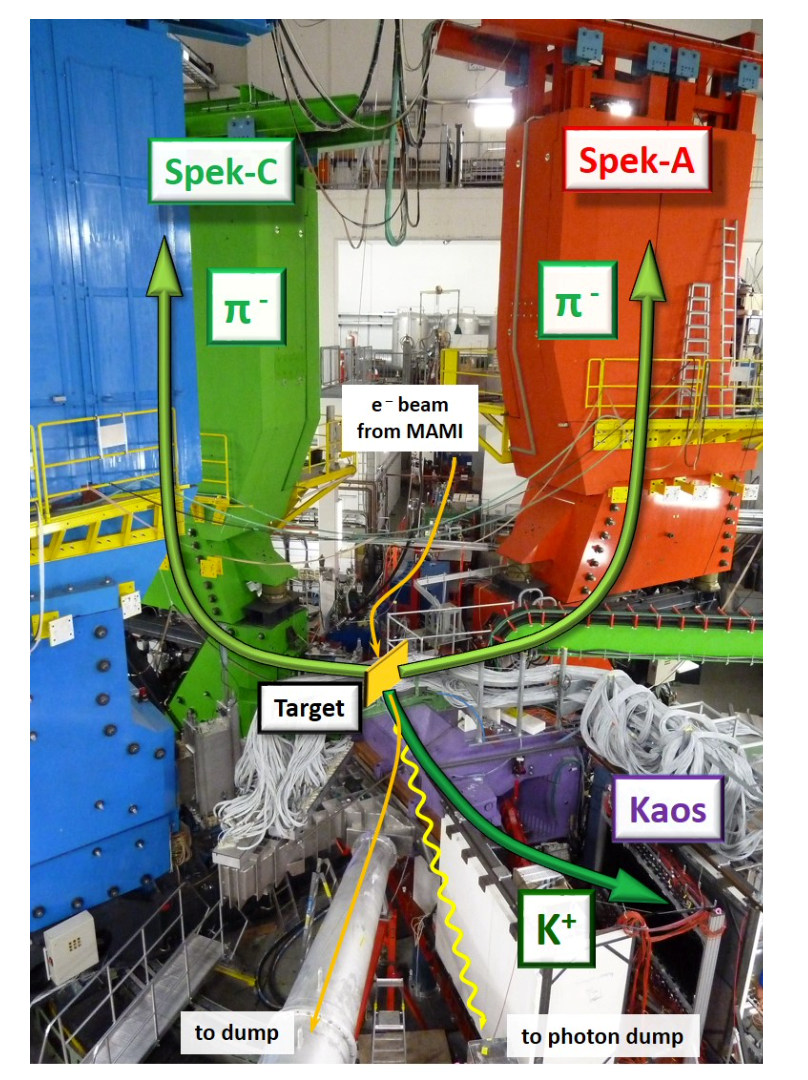
\includegraphics[width=10cm]{image/1-HallA.png}
  \caption[MAMI実験ホール]{A1 Hall概観図。MAMI加速器で加速された電子がビームラインを通って標的チェンバー内の標的に照射される。崩壊パイ中間子法では、照射されて生成されたハイパー核が崩壊する際の$\pi$中間子の運動量を
  Spek A,Cで測定する。またKaosスペクトロメータでは$K^+$中間子の粒子識別を行うことでイベント選択を行う。\cite{esserObservation4Hyperhydrogen2015}}
  \label{exp_hall}
\end{figure}

2014年に行った$^4_{\Lambda}\text{H}$の実験\cite{Schulz2015}では、$\pi$中間子の運動量が
$p_\pi = 132.867 \pm 0.007(\text{stat.}) \pm 0.106(\text{syst.})$ MeV/$c$と測定され、10 keV以下の運動量分解能を実現している(図\ref{fig:pi_spec})。
\begin{figure}[H]
  \centering
  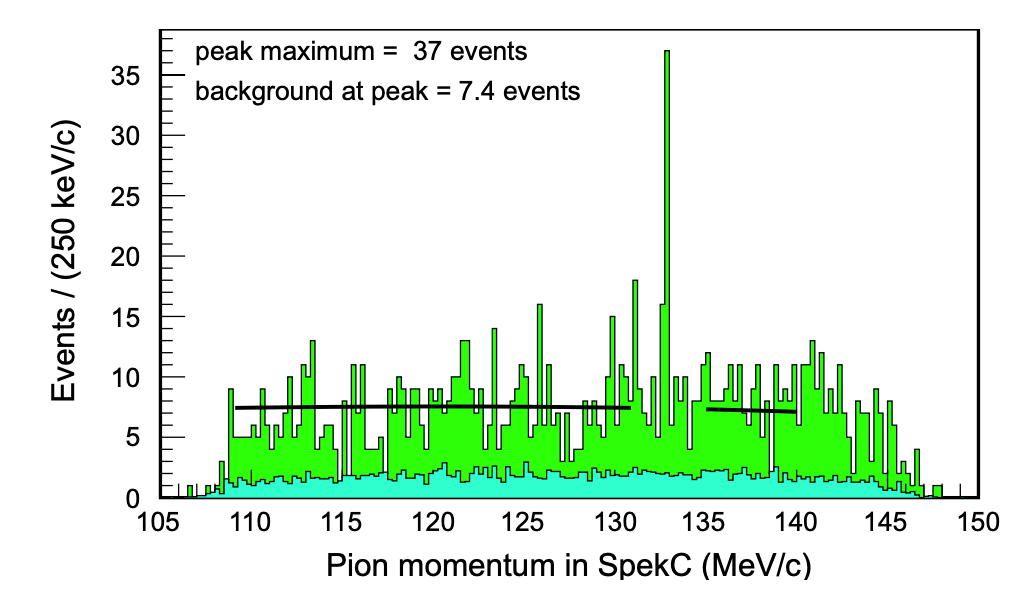
\includegraphics[width=10cm]{image/1-PionSpectrum.png}
  \caption[過去実験での$p_\pi$スペクトル]{高分解能の$\pi$中間子スペクトル。細いピークが133 MeV/c付近に位置しており、これは$^4_{\Lambda}\text{H}$の崩壊で得られる$p_\pi$である\cite{Schulz2015}}
  \label{fig:pi_spec}
\end{figure}

この結果から、$^4_{\Lambda}\text{H}$における$\Lambda$粒子の束縛エネルギー$B_\Lambda$は$B_\Lambda = 2.157 \pm 0.005(\text{stat.}) \pm 0.077(\text{syst.})$ MeVと決定された。

MAMIの持つ高分解能運動量スペクトロメータ(Spek A,C)によって実現される高い分解能は、他のハイパー核質量分光法や重イオン衝突実験では実現できない。
これは崩壊パイ中間子法の大きな特徴であると言える。
ただし、崩壊パイ中間子法は基底状態にのみ適用できるという点で他の手法とは相補的である。

\subsubsection{磁気運動量スペクトロメータ(Spek A, Spek C, Kaos)}
ハイパー核の崩壊に伴う$\pi$中間子の運動量$p_\pi$を測定するためには、MAMIの磁気運動量スペクトロメータを用いる。
実験ホール内のスペクトロメータはSpek A,Cの2つのスペクトロメータと後段のKaosスペクトロメータから構成される。Spek A,Cでは$\pi$中間子の運動量を精密に測定するのに対し、Kaosでは$K^+$を検出することでΛハイパー核が生成されたイベントの選択に用いる。
%Kaosは
運動量測定用のSpek A,C は電磁石と飛跡検出用のドリフトチェンバー、粒子識別用のシンチレーションカウンターとチェレンコフ光検出器から構成されている。
入射した荷電粒子は電磁石によって曲げられるが、その曲率は粒子の運動量に依存する。この性質を利用することで、ドリフトチェンバーによる位置測定の結果から入射粒子の運動量を決定することができる。


\subsection{系統誤差}\label{sec:systematic_error}
10 keVを切る束縛エネルギーの統計誤差に対して、崩壊パイ中間子法の系統誤差は100 keV程度と大きい。
これは$p_\pi$の決定精度に対する系統誤差が100 keV程度あることに由来する。
この節では系統誤差の由来を説明する。

磁気スペクトロメータの運動量絶対値較正のためにMAMIでは電子弾性散乱を利用している。
標的の質量を$m_T$、電子質量を$m_e$、入射電子ビームのエネルギーを$E_{beam}$として、標的で弾性散乱された電子の運動量$p_e'$は散乱角$\theta$に対して一意に決まり、
\begin{eqnarray}
  p_e' = \sqrt{\left(\frac{E_{beam}}{1 + E_{beam}/m_T(1 - \cos{\theta})} \right)^2 - m_e^2}\label{elastic scattering}
\end{eqnarray}
と計算できる。散乱角と入射エネルギーに対する弾性散乱のピーク(図\ref{elastic_scat})から運動量の絶対値を較正する。
ハイパー核の崩壊で放出される$\pi$の運動量はおよそ 100 - 140 MeV/c の領域にあるため、散乱電子も同程度の運動量であることが望ましい。
MAMIの電子線加速器が出せる最低エネルギーである180、195、210 MeVの3種類のエネルギーに対して電子弾性散乱による較正を行っている。
\begin{figure}[h]
  \centering
  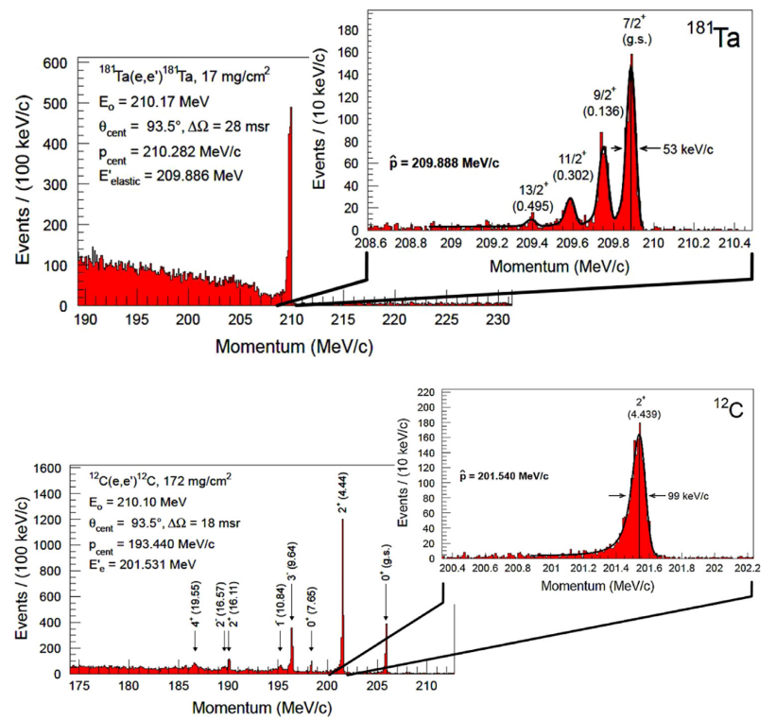
\includegraphics[width=0.8\linewidth]{image/1-elastic.png}
  \caption[電子弾性散乱によるスペクトロメータ較正]{電子弾性散乱によるスペクトロメータ較正実験で得られる散乱電子スペクトル。
  210 MeVで$^{181}\text{Ta}$標的と$^{12}\text{C}$標的を用いて電子弾性散乱を行った例を示している\cite{elastic}。}
  \label{elastic_scat}
\end{figure}


しかしこれまでは200 MeV領域の入射電子ビームエネルギー$E_{beam}$の決定精度が$10^{-3}$つまり200 keV程度と大きかった。式(\ref{elastic scattering})からわかるように散乱電子の運動量の決定誤差のオーダーは
$E_{beam}$の決定誤差と同程度であり、結果的に運動量較正の精度も100 keV/c程度になる。
これが100 keV/cの大きな系統誤差の原因である。電子ビームエネルギーを$10^{-4}$すなわち$20$ keVの精度で決定することができれば、崩壊パイ中間子法の実験全体の誤差を10 keV程度に抑制することができる。

\section{電子ビームエネルギー測定}
\subsection{MAMIにおける従来手法}
MAMIではビームエネルギーを測定するために、偏向電磁石における電子周回軌道の半径を測定する手法が用いられていたが、
これは1.2 GeV領域の電子ビームを100 keV程度の精度で測定し、200 MeV領域の電子ビームエネルギーに外挿することで求める手法であり、
200 MeV領域では20 keV以下の精度を実現することは困難であった。詳細はMAMI加速器の項目(\label{sec:MAMI})で説明する。
%位置を求めてエネルギーを求めている、そして高エネルギーから外挿するから精度がでない
%冨田修論54p

このような背景からいくつかの新しい手法が提案されてきた。
%だから新しい手法が必要
\subsection{逆コンプトン散乱法}
電子ビームエネルギーを直接測定する手法として、逆コンプトン散乱法がある。逆コンプトン散乱法は、電子ビームとレーザー光を衝突させ、
コンプトン散乱で散乱された光子のエネルギーから電子ビームエネルギーを計算する手法である。
レーザー光のエネルギー$E_1$,電子ビームのエネルギーを$\gamma mc^2$,レーザーと電子ビームの衝突角を$\theta$,散乱光子の散乱角を$\phi$として、散乱光子のエネルギー$E_2$は
\begin{eqnarray}
  E_2 = E_1\frac{1+\beta\cos{\theta}}{1-\beta\cos{\phi} + \frac{E_1}{\gamma mc^2} (1-\cos{(\theta +\phi)})} \label{compton}
\end{eqnarray}
と計算できる。電子ビームのエネルギーが高く、レーザー光のエネルギーが十分小さいとして無視できるとき、正面衝突($\theta = 0$)かつ前方散乱($\phi \ll 1$)の場合に散乱光子のエネルギーは最大となり、
\begin{eqnarray}
  E_2 = \frac{4E_1\gamma^2}{1 + \gamma^2\phi^2} \label{compton2}
\end{eqnarray}
と表される。Ge検出器のような$\gamma$線検出器で散乱電子のエネルギーを測定することで、式(\ref{compton2})で表される最大エネルギー領域にコンプトンエッジが現れる(図\ref{fig:comp})。このエッジの位置から電子ビームエネルギーを求めることができる。
\begin{figure}[H]
  \centering
  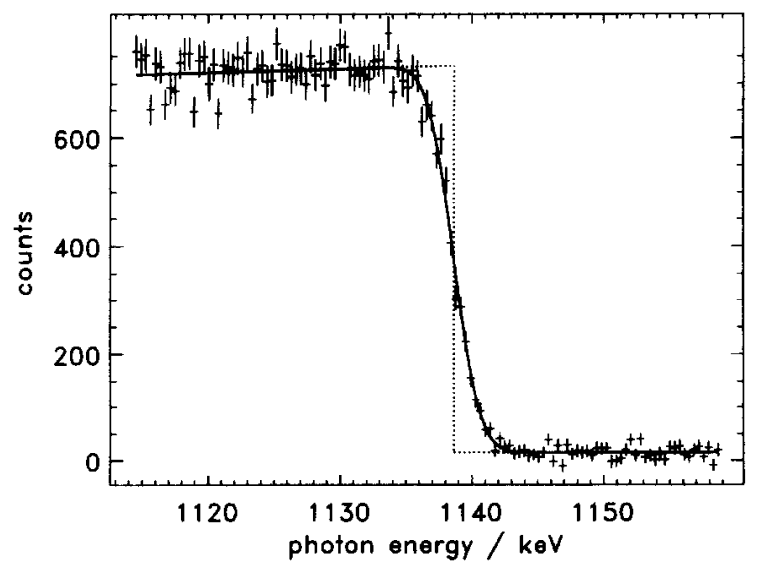
\includegraphics[width=10cm]{image/1-CBS.png}
  \caption[逆コンプトン散乱法]{逆コンプトン散乱法による電子ビームエネルギー測定で得られるコンプトンエッジ\cite{klein1997}}\label{fig:comp}
\end{figure}

しかしこの手法で200 MeV領域の電子ビームエネルギーを測定するには、断面積が小さく、高強度の電子ビームが必要となる。%定量的に書く
MAMI加速器では最大でも30~$\mu$Aの強度の電子ビームしか供給できないが、この時必要な統計量を貯めるには十数時間を要し現実的ではない。
\subsection{偏極電磁石による電子ビームエネルギー測定}
磁場中を運動する荷電粒子は円運動をする。相対論的運動論によれば、磁場$B$中を運動するエネルギー$\gamma mc^2$の電子の運動半径は
\begin{eqnarray}
  r = \frac{\gamma mc}{B}
\end{eqnarray}
である。磁場の精密測定と電子ビームの位置測定によって電子ビームのエネルギーを測定する手法が検討された。
磁場の測定精度および電子ビームの位置決定精度は共に$10^{-4}$の水準を達成しており、電子ビームの決定精度も$10^{-4}$の精度で決定できることが実証された。
しかしこの手法は180 MeVの電子ビームでの実証にとどまっており、195 MeVや210 MeVの電子ビームでは十分な精度を得ることができなかった\cite{herrmann}。
\subsection{アンジュレータ放射光干渉法の開発の経緯}
崩壊パイ中間子法の系統誤差を抑えるためには、200 MeV領域の電子ビームエネルギーの高精度測定が必要であるが、
従来の手法や既知の手法では十分な精度を得ることができなかった。
そこで我々は2016年からアンジュレータによる放射光を用いた電子ビームエネルギー較正手法(アンジュレータ放射光干渉法)の開発に取り組んできた\cite{klag2018,klag2023}。
本研究の目的はアンジュレータ放射光干渉法を用いて電子弾性散乱によるスペクトロメータ較正実験を行い、$10^{-4}$以上の電子ビーム絶対値較正精度を達成することである。
\end{document}